\documentclass[pdflatex,sn-apa]{sn-jnl}% Springer Nature template, APA (author--year) reference style

\usepackage{graphicx}
\usepackage{amsmath,amssymb,amsfonts}
\usepackage{amsthm}
\usepackage{float}
\usepackage[title]{appendix}
\usepackage{xcolor}
\usepackage{textcomp}
\usepackage{booktabs}

\newtheorem{lemma}{Lemma}
\newtheorem{proposition}{Proposition}
\newtheorem{corollary}{Corollary}
\theoremstyle{definition}
\newtheorem{definition}{Definition}
\providecommand{\E}{\mathbb{E}}
\providecommand{\R}{\mathbb{R}}
\providecommand{\cA}{\mathcal{A}}
\providecommand{\cO}{\mathcal{O}}
\providecommand{\cS}{\mathcal{S}}
\providecommand{\cW}{\mathcal{W}}
\providecommand{\Emp}{\mathfrak{E}}
\providecommand{\Capa}{\mathsf{C}}
\providecommand{\KL}{D_{\mathrm{KL}}}

\raggedbottom

\begin{document}

\title[Characterising Agency in Active Inference]{Characterising Agency in Active Inference: An Empowerment Probe and Structure Learning with Tensor Networks}

% Double-blind review: author names, affiliations, acknowledgements and declarations
% are on the separate title page (titlepage.tex), not in this manuscript.

\abstract{The spread of agentic artificial intelligence has outpaced the conceptual tools for characterising computational agency. We argue for a minimal notion built on three criteria: intentionality as action grounded in beliefs and desires, rationality as action that follows coherently from a model of the world, and explainability as action causally traceable to internal states. We implement these criteria in an active inference agent acting in a partially observable Markov decision process, in which beliefs, preferences and the minimisation of expected free energy form a chain that leads to action, and compare it with belief--desire--intention architectures and model-based reinforcement learning. In a minimal T-maze, we measure control with empowerment, the maximum information an agent's actions can carry into its next observations. Structural manipulations of the generative model yield zero-, intermediate- and maximal-control regimes. We prove that learning never lowers the agent's expected estimate of its empowerment, as long as its available actions and observations stay the same. An action taken to gain information therefore raises empowerment exactly when it leaves those actions and observations in place. Minimising expected free energy selects that action through preferences or through the drive to gain information; empowerment is never itself an objective. Tensor networks learn the generative model from behaviour and reproduce the control regimes. Structure learning recovers the four hidden states we specified for the minimal maze, discovers seven in the pymdp T-maze, and shows that behaviour does not support the context variable our information-gain analysis assumes. We close with falsifiable governance hypotheses.}

\keywords{Agency, Active inference, Empowerment, Epistemic action, Structure learning, Tensor networks}

\maketitle

\section{Introduction}\label{Introduction}

Agency is now the central term in artificial intelligence (AI). Generative AI predicts well from historical data and has clear limits. It lacks a world model~\citep{lecunPathAutonomousMachine2022}, does not reason in real time, and handles novel scenarios poorly. Much current work therefore aims at models that understand the world and act independently. Commercial applications are heading the same way under the name of \emph{agentic workflows}~\citep{ngAgenticDesignPatterns2024}, and \emph{agentic} AI is the label under which increasingly autonomous systems are now designed and deployed.

If the promise of agentic AI rests on systems that \emph{act} and do not merely execute, then tools for defining and measuring agency become a prerequisite for both engineering and oversight. We hold that AI agency involves reasoning, autonomy, explainability and governance at once. Addressing it requires a definition rich enough to capture the dimensions of agency we recognise in humans yet simple enough to measure in AI systems. It also requires a computational architecture that implements that definition. This paper argues that active inference, developed in theoretical neurobiology~\citep{parrActiveInferenceFree2022a}, meets both requirements.

A methodological advantage of active inference is that it supports the practice known as ``computational phenotyping'' in computational psychiatry~\citep{montagueComputationalPsychiatry2012,schwartenbeck2016computational,smithStepByStep2022}. Operationally, phenotyping fits a generative model to behavioural data and then uses the inferred parameters to explain variation across individuals or conditions. By analogy, if active inference also maps the basic structure of agency, the same procedure could phenotype the computational traits that qualify an AI system (active inference-based or otherwise) as being endowed with agency. The worked example in this paper performs the second half of this programme on manually specified models. Section~\ref{sec:learned} takes the first step on learned models. Tensor networks fitted to behaviour alone recover the hidden states we specified for the minimal maze and discover those of the pymdp T-maze, for which we specified none. They also show that the context variable on which our information-gain analysis rests is not a hidden state that behaviour supports. The same section shows which parts of the hand-specified account behaviour can certify.

Section~\ref{sec:definition} motivates the definition and situates it against prior work, Section~\ref{sec:worldmodels} instantiates it in active inference, Section~\ref{sec:worked} develops the T-maze example, the empowerment probe and the learned-model pipeline, and Section~\ref{sec:discussion} recasts the governance implications as hypotheses.

\section{A Simple, But Not Too Simple Definition of AI Agency}\label{sec:definition}
\subsection{Why the Current Definition of AI Agency Is Not Enough}

The agents literature has never lacked distinctions. \citet{wooldridgeIntelligentAgentsTheory1995} separated a weak notion of agency (autonomy, social ability, reactivity, pro-activeness) from a strong one that adds belief, intention, obligation and emotion; \citet{stoneMultiagentSurveyML2000} and \citet{jenningsRoadmapAgentResearch1998} organised the field around reactive, deliberative and social agents and their learning; and the BDI tradition (Section~\ref{sec:priorwork}) gave the strong notion formal and executable content. What the wider AI community inherited, however, is the weak definition~\citep{luckConceptualFrameworkAgent2001}. In current usage ``agentic'' has narrowed further to autonomy of execution plus goal-directedness, often reduced to linear autonomy scales (e.g.,~\citep{shavitPracticesGoverningAgentic}, the SAE Levels of Driving Automation~\citep{vyasKeySafetyDesign}, ALFUS~\citep{huangAutonomyMeasuresRobots2008}). Our claim concerns that inherited operational definition and leaves the tradition that produced it untouched. \citet{franklinAgentOrProgram1997} gave the standard taxonomy of what separates an agent from a program, and \citet{floridiMoralityArtificialAgents2004} proposed interactivity, autonomy and adaptability as a three-criterion definition; ours takes the mental-state structure as the object of the definition, where theirs takes the behavioural profile.

Such levels oversimplify autonomy, which has multiple dimensions~\citep{staytonItsTimeRethink2020}. A robot may be autonomous in navigation yet rely on humans for goal-setting. As NIST notes, autonomy measures must serve many audiences and dimensions~\citep{huangFrameworkAutonomyLevels2005} many of which align with the strong definition's criteria (knowledge, beliefs, intentions, emotions, obligations). Autonomy and goal-directedness cannot fully capture agency. In an agent that is embedded in its environment, reacting and taking initiative are hard to separate, and the ``inessential'' properties of the strong definition may not be so inessential, since our intuitions about agentic behaviour extend beyond merely ``autonomous'' conduct. A satisfying definition should balance strong and weak criteria without anthropomorphism.

\subsection{Rationality, Intentionality, and Explainability}

Philosophical accounts of agency help in reaching a parsimonious definition. At its core, agency implies the capacity for intentional action, that is, the ability of an actor to initiate and direct events. Following \citet{davidsonEssaysActionsEvents1980}, agency is the capacity to act rationally and intentionally. Acting rationally means achieving an outcome that follows from standards of rationality. Acting intentionally means acting in accordance with mental states (beliefs, desires, intentions or plans) from which the intended outcome is derived and whose options one can ``weigh''. These mental states should also ``cause'' the action. That causal link makes the action explainable, since it exposes the mental states behind it.

On this view, agency is the capacity to perform actions that are intentional, rational and explainable. ``Turning on the light'' to ``get to the fridge'' because ``you want to eat'' and ``believe the fridge is in the kitchen'' both qualifies one as an agent and allows another to explain the action.

But what about autonomy? Philosophers disagree on its precise meaning. Classical traditions (Kantian, Millian) frame it as the capacity to live by self-chosen reasons, while relational~\citep{oshanaRelationalAutonomy2020} and feminist theories~\citep{mackenzieFeministConceptionsAutonomy2017} re-cast it as procedurally defined by authenticity of one's choices. Despite disputes, autonomy always traces back to independence of action, itself tied to an agent's intentions, beliefs, and desires. An action performed on behalf of another is not fully autonomous, as it conforms to the other's mental states. Autonomy and intentionality are not identical. A system may execute independently without acting on anything like its own beliefs and desires. The independence that matters for autonomy is independence of the mental states from which action comes. We therefore treat intentionality as the central notion in what follows, and use ``autonomy'' as shorthand for intentional independence of action, without treating it as a separate criterion.

Another concept often tied to agency is adaptivity, the capacity to maintain adequate performance as the environment changes. It is closely related to rationality~\citep{shavitPracticesGoverningAgentic}. Both rely on learning and updating a world model, a structure that links mental states to states of the world and can represent what would happen under different actions.

\subsection{Relation to Prior Work}\label{sec:priorwork}

Our three criteria are stated independently of any implementation, so they can be applied across agent architectures; doing so both situates our proposal in prior work and guards against circularity (the worry that active inference satisfies the criteria merely by definition).

Belief--desire--intention (BDI) architectures~\citep{bratmanIntention1987,cohenIntentionChoiceCommitment1990,raoModelingRationalAgents1991,raoBDIAgents1995} are the closest ancestors of our proposal. They give beliefs, desires and intentions explicit representations with a formal semantics (branching-time possible-worlds models in~\citet{raoModelingRationalAgents1991}, the logic LORA in~\citet{wooldridgeReasoningRationalAgents2000}) and an operational reading in agent programming languages~\citep{bordiniProgrammingMultiAgentJason2007,dastani2APL2008,boissierJaCaMo2013}, so they satisfy intentionality by construction and are highly inspectable. Uncertainty is not foreign to the tradition. Intention reconsideration has been treated decision-theoretically~\citep{schutIntentionReconsideration2004}, BDI plans have been mapped to MDP policies and back~\citep{simariMDPsBDI2006}, hybrid BDI--POMDP architectures use team plans to make POMDPs tractable and POMDP analysis to improve the plans~\citep{nairHybridBDIPOMDP2005,bautersAgentSpeakPOMDP2016}, graded BDI models carry degrees of belief, desire and intention~\citep{casaliGradedBDI2011}, and plan-selection context conditions can be learned from experience~\citep{singhLearningContextBDI2010}. What these integrations share is that the probabilistic component is attached to a deliberation cycle whose control structure (option generation, filtering, commitment) is specified separately from it. BDI handles uncertainty well. The difference we draw is that it does not derive perception, action selection and uncertainty handling from a single objective, so rationality is assessed relative to the commitment strategy in force and there is no one quantity the whole architecture minimises. Model-based reinforcement learning (e.g.,~\citep{hansenTDMPC2ScalableRobust2024}) inverts this profile. It possesses an explicit normative objective (expected return) and a world model, but desire-like states are collapsed into a scalar reward, and learned latent states are rarely semantically transparent; both intentionality (in the belief--desire sense) and explainability suffer as a result. End-to-end deep policies satisfy none of the three criteria transparently~\citep{liptonMythosModelInterpretability2018}; the post-hoc explainability literature~\citep{arrietaExplainableAI2020} attaches explanations to such systems from the outside, which is categorically different from an architecture whose internal variables natively play belief-like and desire-like roles. BDI matches active inference on intentionality and model-based RL matches it on rationality. What active inference adds, we will argue, is that one objective, expected free energy, delivers all three criteria together with calibrated uncertainty. Section~\ref{sec:learned} further shows that our operational probe does not presuppose active inference. It applies to any system for which a generative model of the sensorimotor stream can be obtained. A causal definition of agency, on which a system is an agent if it would adapt its policy when its actions influenced the world differently, has been proposed and turned into a discovery algorithm by \citet{kentonDiscoveringAgents2023}. It is the closest formal alternative to our criteria. It tests whether the policy adapts to the mechanism; our criteria also ask that the adaptation run through inspectable beliefs and preferences, and this makes the third criterion, explainability, checkable. Active inference has also been extended to interacting agents and to the formation of shared beliefs across a population~\citep{albarracinEpistemicCommunities2022}. The present paper concerns the single-agent case and leaves multi-agent controllability, where one agent's empowerment is another's constraint, to future work.

\begin{table*}[t]
\centering
{\small
\begin{tabular}{|p{2.2cm}|p{2.8cm}|p{2.8cm}|p{2.8cm}|}
\hline
\textbf{Architecture} & \textbf{Intentionality} & \textbf{Rationality} & \textbf{Explainability} \\
\hline
BDI~\citep{raoBDIAgents1995,wooldridgeReasoningRationalAgents2000} & Explicit beliefs, desires, intentions with formal semantics & Normative at the level of commitment strategies; decision-theoretic and POMDP extensions exist~\citep{schutIntentionReconsideration2004,nairHybridBDIPOMDP2005}, but no single objective spans perception, deliberation and action & High; symbolic states inspectable \\
\hline
Model-based RL~\citep{hansenTDMPC2ScalableRobust2024} & Partial; desires collapsed into scalar reward & Normative objective (expected return) & Partial; learned latents rarely interpretable \\
\hline
End-to-end deep policies & Absent as explicit structure & Implicit at best & Post-hoc only~\citep{arrietaExplainableAI2020} \\
\hline
Active inference & Posteriors (beliefs) and prior preferences (desires) & Normative objective (expected free energy), bounded, uncertainty-calibrated & High; probabilistic roles and precisions inspectable \\
\hline
\end{tabular}
}
\caption{The three criteria of agency applied across agent architectures. Cells summarise how, and whether, each criterion is realised natively by the architecture.}
\label{tab:frameworks}
\end{table*}


\section{World Models in Active Inference and Agency}\label{sec:worldmodels}

\subsection{World Models and Agency}

A useful definition of AI agency, simple but not too simple, should include the following criteria:

\begin{enumerate}
    \item \textbf{Intentionality/autonomy}: The ability to ground one's actions in one's own mental states such as beliefs, desires, intentions or plans;
    \item \textbf{Rationality/adaptivity}: The ability to make decisions that rationally (e.g., logically or probabilistically) follow from one's understanding of the world.
    \item \textbf{Explainability}: The ability for an observer to explain the system's action as causally related to its mental states and understanding of the world.
\end{enumerate}

The pairings follow Section~\ref{sec:definition}. Autonomy is treated as intentional independence of action, and adaptivity as the behavioural signature of rationality under an adequate world model. All three attributes can be meaningfully expressed as attributes of actions performed by systems endowed with agency, and all appear to be traceable to a detailed understanding of the world. In AI, such an understanding can be derived from a ``world model''. Whether it \emph{must} be so derived remains an open question; our claims are restricted to architectures where it is. There have been many proposals of ``world models'' for AI, especially in the last few years, and many of them are ``explainable'' in virtue of their transparent architecture. But few of them express clearly the relation between the intentionality and rationality criteria of agency defined above.


\begin{figure}[t]
\centering
\includegraphics[width=0.75\columnwidth]{Fig1.png}
\caption{The agentic action chain in an active inference world model. Beliefs (posteriors over hidden states, updated by evidence) and desires (prior preferences over observations) are shown as blue boxes. Both enter the expected free energy, whose minimisation (green arrow) selects the action.}
\label{fig:rationality-intentionality}
\end{figure}

In a recent extensive review, \citet{dingUnderstandingWorldPredicting2024} categorise world models into those that construct internal representations of how the external world works to support decision-making, and those that predict its future states from perceptual input.

The active inference models we present fall under Ding et al.'s first category, specialised for decision making, alongside Reinforcement Learning (RL) and MDP-based approaches. The active inference Partially Observable MDPs (POMDPs)~\citep{dacostaActiveInferenceDiscrete2020} we focus on are close in spirit to RL but differ by not specifying a reward function (for comparisons, see~\citep{tschantzREINFORCEMENTLEARNINGACTIVE2020,fristonReinforcementLearningActive2009a,dacostaRewardMaximizationDiscrete2023}). They are of particular interest here. They are clear examples of world models that both represent and predict. They lend themselves to computational phenotyping. Their parameters and inference processes also map directly onto the criteria of agency above, since beliefs and preferences combine to drive action selection in a way an observer can follow (Fig.~\ref{fig:rationality-intentionality}).

\subsection{Active Inference's World Models}

An active inference world model consists of the state transition matrix and the likelihood matrix of a POMDP. The transition matrix gives the probability of moving between hidden states, and the likelihood matrix gives how reliably each state produces each observation. These form the POMDP about the world, congruent with other learned world models such as UPDP~\citep{duLearningUniversalPolicies2023} or TD-MPC2~\citep{hansenTDMPC2ScalableRobust2024}. Modelling the world is an intrinsic part of an active inference agent, which cannot proceed without some belief (however correct) about the world. The model need not be accurate. Agents break possibly continuous inputs into discrete categories, which then form the basis of reasoning. Once categories are created, the world can be mapped from observations to hidden causes and coarse-grained into hierarchical levels. Likelihood mappings aggregate to longer and larger spatio-temporal scales, which translate to the transition matrices.

\subsection{Intentionality, Rationality, and Explainability in Active Inference}

\subsubsection{Intentionality.}
In philosophy of action, intentionality is understood through a belief--desire model. An agent acts intentionally when its behaviour is caused by its beliefs about the world and its desires about how the world ought to be. For Humeans, beliefs aim to represent reality (mind-to-world fit), whereas desires aim to change it (world-to-mind fit)~\citep{smithHumeanTheoryMotivation1987}. Debates exist over whether this distinction can be collapsed~\citep{junker2024predictive}.

Active inference preserves this structure. In a variational POMDP formulation, belief-like states are encoded in the agent's posterior over hidden states and model parameters, while desire-like states are encoded as prior preferences over observations. Preferences are implemented as log-prior probabilities over sensory states, so an agent can hold beliefs about state $s$ while desiring outcome $o$. This tension drives policy selection through expected free energy minimisation~\citep{parrActiveInferenceFree2022a}, which gives the intentional stance~\citep{dennettIntentionalStance1987} a computational reading. An active inference agent acts to reduce the gap between predicted and preferred outcomes, which is the Humean belief--desire structure written in probabilities. Because preferences are represented explicitly, the agent is fully representational and escapes the ``desert landscape'' objection that predictive accounts of the mind leave no room for desire-like states~\citep{williamsDesertLandscape2018}.

\subsubsection{Rationality}
Rationality concerns the coherence of actions with beliefs and goals. An active inference agent selects policies by minimising expected free energy, an objective that contains classical expected utility maximisation~\citep{dacostaRewardMaximizationDiscrete2023} and adds a formal account of exploration, so both instrumental rationality (pursuing preferred outcomes) and epistemic rationality (reducing uncertainty) follow from it. The rationality is bounded~\citep{simonModelsMan1957,ortegaThermodynamicsFreeEnergy2013}, so the agent is optimal relative to its model and its computational limits, and unexpected behaviour traces back to mis-specified beliefs, preferences or model assumptions. The criterion has two parts, coherence of action given the model and adequacy of the model given the environment.

\subsubsection{Explainability}
Explainability concerns understanding why a system took a particular action. Active inference is explainable because its probabilistic structures are explicit, beliefs as posteriors, preferences as priors, predictions as the likelihood mapping and policies as action sequences, and an observer can inspect them to reconstruct an action mechanistically and semantically. Because the posteriors carry their own uncertainty, an observer can also read off how confident the agent was and how it traded exploitation against exploration. Interpretability of this kind is intrinsic to the architecture~\citep{albarracinVariationalApproachScripts2021}, and structured generative models with disentangled latent states push it further toward ``monosemantic'' planning representations~\citep{brickenMonosemanticity2023}. An observer can follow the agentic action chain:

\begin{center}
belief updating (beliefs) $\to$ computation of expected free energy weighted by preferences (desires) $\to$ policy selection $\to$ action
\end{center}

It is the causal chain from mental states to action that Davidson's account requires.

\section{Worked Example of Agency Phenotyping}\label{sec:worked}

We present a minimal T-maze example in which an agent's intentionality, rationality and explainability are varied through the agentic action chain and tracked with empowerment (Section~\ref{sec:metric}). This is a controlled illustration. Generative models are manually specified, and we verify that the probe tracks known structures where ground truth is available; Section~\ref{sec:learned} then learns the models from data. The example shows that differences in the generative model produce quantifiable control regimes, that empowerment probes control capacity, and that epistemic action and empowerment interact. It also asks which governance controls remain effective as agents gain intentionality, rationality and explainability.

\subsection{The Task}

We investigate the minimal T-maze (Fig.~\ref{fig:tmaze}), formalised as a discrete two-step POMDP \footnote{The standard pymdp T-maze splits observations into three modalities whose product yields 24 outcomes, so empowerment is maximal already at $t_1$. We use the minimal variant for economy of exposition, and restrict empowerment to the relevant modalities when replicating in the pymdp T-maze.}. The agent has three actions: Left, Right and Cue (Down), and four possible observations: Cheese, Shock, Left and Right. Cheese and shock are randomly placed left vs.\ right with 50/50 probability, and the observation at the Cue reveals their location. Going Right or Left leads to an absorbing state, a trap the agent cannot leave. Any subsequent action yields the same observation as at time step 1. The optimal solution is to visit the Cue first and then the cheese (assuming one has a preference for cheese and an aversion to shock). We restrict the agent to a planning horizon of one time step, so that it evaluates only the consequences of its next action; every action at the choice point yields one bit about the cheese location, and the Cue is selected because it is the one informative action whose outcomes the agent is not averse to (Section~\ref{sec:efe}).

\begin{figure}[t]
\centering
\includegraphics[width=0.75\columnwidth]{Fig2.png}
\caption{The T-maze task. Shown are the two possible initialisations of the environment. The arrow symbolises the observation Right or Left and points to where the cheese is.}
\label{fig:tmaze}
\end{figure}

The task suits our purpose because it contains uncertainty that every action resolves, one action (Cue) that resolves it while preserving control, two (Left/Right at $t_1$) that resolve it and lose control, and a natural distinction between agents that seek information and agents that do not. Differences in rationality and intentionality show up in that distinction.

\subsection{The Metric}\label{sec:metric}
Empowerment measures the degree of control an agent has at a given location in an environment. It is defined as the channel capacity between actions and their consequences \citep{Klyubin2005empowerment,salgeEmpowermentIntroduction2014,mohamedVariationalInformationMaximisation2015}, that is, the maximum mutual information between a set of actions $A_t$ at time $t$ and a set of future observations $O_{t+1}$ at time $t+1$, taken over all possible action distributions $p(a_t)$. We call the freedom to range over all such distributions the \emph{free choice assumption}.

\begin{align}
\text{Empowerment}_t &= \underset{p(a_t)}{\max}\ I(A_t ; O_{t+1}) \\
 &= \underset{p(a_t)}{\max}\sum_{a_t, o_{t+1}} p(o_{t+1}|a_t)\, p(a_t) \nonumber\\
 &\qquad\quad \times \log_2 \frac{p(o_{t+1}|a_t)}{\sum_{a'_t} p(o_{t+1}|a'_t)\, p(a'_t)}
\end{align}
We have omitted the conditioning of empowerment on a current state or location in the environment for clarity. We have expanded the definition of the mutual information in (2) to show that empowerment is a function of the conditional $p(o_{t+1}|a_t)$ alone.

Why maximise over $p(a_t)$? Empowerment is a channel capacity. It asks how many distinguishable ``messages'' an agent could, in the best case, send into its future observations through its actions. Maximising over action distributions makes the quantity a property of the agent--environment interface at a state, independent of any particular policy. By interface we mean the set of actions available at that state and the observations they can produce. This is the purpose of the free choice assumption, and it comes at a cost. The measure describes the control available to an idealised agent free to deploy any action distribution. The actual agent exercises less, because its preferences and habits restrict the choice of $p(a_t)$ (see \emph{potentiality vs.\ actuality} below). The measure also ignores the agent's policy. A uniformly random controller occupies states with exactly the same potential empowerment as a deliberative planner.

Empowerment has a cybernetic ancestry. \citet{wienerCybernetics1948} treated control and communication as one problem. \citet{ashbyIntroductionCybernetics1956} showed that a regulator can hold a variable within bounds only if it commands at least as much variety as the disturbances it faces, and \citet{touchetteInformationTheoreticLimits2000,touchetteInformationTheoreticControl2004} gave that law its information-theoretic form, with controllability and observability written as conditional entropies. Empowerment~\citep{Klyubin2005empowerment,klyubinKeepYourOptions2008} is the capacity of the actuator-to-sensor channel, the variety an agent can inject into its own future observations, and so belongs to the same family of quantities. \citet{conantGoodRegulator1970} is a different result, that a maximally simple successful regulator must be a model of what it regulates. Our rationality criterion assesses action relative to an explicit world model, which is close to that reading without being identical to it, and the use of the good-regulator theorem in support of Bayesian accounts of control has been questioned~\citep{baltieriWattGovernors2020}. We take two things from this tradition, a measure of control capacity and a criterion of rationality relative to a model, and the T-maze example applies both.

\subsubsection{Objective vs Subjective.} The conditional $p(o_{t+1}|a_t)$ captures the effect of an action on its subsequent observation. If it is the \emph{true} transition distribution of the environment, the channel capacity measures the control an agent \textbf{could have in principle}. We term this \textbf{objective empowerment}. If the conditional is instead the agent's \emph{belief} about the transition probabilities, the channel capacity measures the control the agent \textbf{believes it has}. We call this \textbf{subjective empowerment}. Researchers have access to the true conditional in small simulated environments but typically not in large ones; in explainable models like POMDPs the subjective conditional is accessible, and subjective empowerment is a continuous function of the beliefs, so it approaches objective empowerment as the beliefs approach the true conditional.

\subsubsection{True empowerment.} Ideally one would want neither what is possible in an environment nor what the agent believes is possible, but what the agent \textbf{can actually do}, which we call \textbf{true empowerment}. An operational definition must account for two deviations from the idealisation. The first is erroneous belief, which separates objective from subjective empowerment. The second is violation of the free choice assumption, where goals and preferences constrain the action space, and it yields a second categorisation.

\subsubsection{Potentiality vs Actuality.} Under the free-choice assumption, the formula measures what an agent \textbf{potentially could do}, its \textbf{potential empowerment}. Once the agent selects actions by optimising an objective (reward in RL, free energy in active inference) or carries a particular preference distribution, the available action distributions shrink and empowerment with them. In Polani's football example, a player in possession of the ball has high potential empowerment over where it goes next, but when standing before an open goal, the preference for scoring leaves only one option, so their \textbf{actual empowerment} is smaller. Section~\ref{sec:efe} gives one precise version, actual empowerment under the agent's own policy. Goal-directed empowerment~\citep{goalDirectedEmpowerment} is a related construction.

\subsubsection{Our choice of metric.}
Lacking an operational definition of true empowerment, we restrict ourselves to the forms we can compute. The four variants above are two orthogonal axes, objective versus subjective (whose conditional enters the channel) and potential versus actual (whose action distribution is used), and the quantity we compute throughout is subjective potential empowerment. Our main claim, connecting empowerment to active inference, concerns epistemic action. An epistemic action is an action taken to reduce uncertainty, either about hidden states (active inference) or about model parameters (active learning~\citep{schwartenbeck2019activelearning}). One might expect such an action to lead to a state of higher empowerment. In general it does not. In the maze below, entering an arm resolves where the cheese is just as the Cue does, and leaves the agent in a state with no control at all. Proposition~\ref{prop:epistemic} therefore separates what an action reveals from where it leaves the agent.

\begin{proposition}[When epistemic action raises empowerment]\label{prop:epistemic}
Write the expected change in subjective potential empowerment produced by an action as the sum of an information term (the change due to updating the belief, at the interface the agent starts from) and an interface term (the change due to moving to a new interface, evaluated at the updated belief). The information term is never negative, because channel capacity is convex in the channel and the channel predicted under a mixed belief is the expectation of the channels predicted under each resolved belief, so Jensen's inequality applies. The interface term has no sign. An action raises expected empowerment whenever it resolves hidden-state uncertainty without degrading the interface, in particular whenever it returns the agent to the same choice point.
\end{proposition}

The decomposition and proof are in Appendix~\ref{app:proofs}. Section~\ref{sec:noisyarm} checks the decomposition numerically on a grid of noisy channels, where the information term is never negative and each arm's net change is minus one bit.

The proposition concerns one particular quantity. Subjective potential empowerment is the capacity of the belief-averaged channel, the single conditional $p(o_{t+1} \mid a_t)$ that an agent with belief $q$ predicts and plans with. The information term equals the difference between that capacity and the belief-expected capacity $\E_{s \sim q}[\Capa(W_s)]$, the gap that Jensen's inequality bounds. One could instead define empowerment as this expected capacity, the average of the empowerment the agent would have in each possible world. Under that definition the term is zero by linearity, so gaining information has no effect on empowerment. We use the capacity of the mixed channel because the agent's own predictive model outputs it. The expected capacity needs access to the resolved worlds, which belongs to the objective side of the distinction drawn above. In plain terms, uncertainty makes the predicted outcomes of different actions look more alike, so an agent planning with its predictions underestimates its control. An epistemic action restores that amount, provided the agent's available actions and observations remain.

Learning more about the environment raises the control the agent computes it has, as long as the learning does not remove the actions it would use. We demonstrate both cases in the minimal T-maze by fixing the agent's transition beliefs to the true distribution (so subjective and objective empowerment coincide), with a preference for cheese and an aversion to shocks. The Cue resolves the context and returns the agent to the same three-way choice, so its interface term is zero and empowerment rises. Either arm resolves the context equally well but enters an absorbing state, so its interface term is negative and empowerment falls. Actual empowerment is too narrow for stating the proposition, though it is the right quantity for phenotyping agents (Section~\ref{sec:efe}). Using subjective potential empowerment as our metric, we show that a free-energy minimising agent with the standard preferences takes the interface-preserving epistemic action. Empowerment maximisation need not be added as an explicit objective, since minimising free energy already yields accurate beliefs and, under those preferences, actions that preserve the capacity to form them. \citet{hafnerActionPerceptionDivergence2020} place empowerment and expected information gain on one spectrum of objectives. The observation here is narrower. In this task the standard active inference objective already selects the empowering action without an empowerment term.

\subsubsection{What empowerment does and does not measure.}\label{sec:notagency}
Empowerment quantifies how well the observations that follow an agent's actions tell those actions apart, that is, how many distinct futures the actions can reliably select among. It measures \emph{controllability}. It does not measure agency as defined in Section~\ref{sec:definition}, and the two come apart in both directions. A random-action controller occupying an empowered state has high potential empowerment with no beliefs, preferences or world model at all. A model-based planner with a narrow actuator interface can satisfy all three criteria and still have low empowerment; for such a system empowerment bounds how much of its agency it can \emph{express}. We use empowerment as a probe of the control capacity that intentional action presupposes. The three criteria are assessed on the agent's internal states, its beliefs, its preferences and their causal role in action selection, all of which can be inspected in an explicit generative model. Empowerment tracks whether the environment and the available actions leave those states anything to decide. If empowerment is zero at every horizon up to the planning horizon, the agent still has agency but it has no observable effect, since nothing the agent believes or wants can then make a difference to what it observes. High empowerment is necessary for high agency and does not guarantee it.

\begin{proposition}[Zero empowerment silences agency]\label{prop:zero}
Let $T$ be the planning horizon and let $n$-step empowerment be the capacity from length-$n$ action sequences to length-$n$ observation sequences (Appendix~\ref{app:proofs}). If $n$-step empowerment is zero for every $n \le T$, then every policy, open- or closed-loop, induces the same distribution over observation sequences of length $T$, so no belief or preference can make an observable difference within the horizon. Zero one-step empowerment does not suffice. Two actions with identical immediate consequences can lead to hidden states that a later observation distinguishes, so one-step empowerment can be zero while two-step empowerment is a full bit.
\end{proposition}

The T-maze trap below is absorbing, so its empowerment is zero at every horizon and the proposition applies in full. Empowerment values can be read as agency regimes there only because the agentic action chain is independently in place and inspectable. Without it the same numbers would report controllability alone.


% \subsection{The Model}






% \begin{equation}
% \text{Empowerment}_t = \max_{p(a_t)} I(A_t ; O_{t+1})
% \end{equation}


\subsection{Empowerment along the task}

We compute the subjective potential empowerment at $t_1$, and then at $t_2$ in two cases, after the agent has gone Left or Right first and after it has gone to the Cue. Fig.~\ref{fig:likelihood-pre} displays the agent's manually fixed beliefs at the first time step. In this minimal setting any two actions either predict exactly the same distribution over observations or predict observations that never overlap. The empowerment values, computed with the Blahut--Arimoto algorithm (the standard iterative method for channel capacity), therefore equal $\log_2 k$, where $k$ is the number of actions with distinct predictions. The formula holds only for that structure. If two actions predict different but overlapping distributions, the capacity can fall below $\log_2 k$. It can also exceed $\log_2 k$, for example when one action's outcomes overlap those of two others and also include an outcome neither of them produces. These values are unsurprising. They come from the same generative model that realises the belief--desire--action chain, so they can be read alongside it.

\begin{figure}[t]
\centering
\includegraphics[width=0.75\columnwidth]{Fig3.png}
\caption{Transition distribution $p(o_2\mid a_1)$ at the first time step. Left and Right produce indistinguishable observation distributions, so they are effectively one action, as far as empowerment is concerned. The agent has 2 of the possible 3 distinct actions at its disposal, so empowerment is not yet maximal.}
\label{fig:likelihood-pre}
\end{figure}

\subsubsection{Baseline Empowerment at $t_1$ (Intermediate-Control Regime, $\log_2 2=1$ bit).}

Before taking any action, the agent's subjective potential empowerment at time $t_1$ is 1 bit, or $\log_2(2)$. Although the agent nominally has three actions, it effectively perceives only two distinguishable control options (Cue vs.\ either terminal choice). Submaximal empowerment, a value above 0 and below the maximum, marks an intermediate-control regime. The agent has nonzero influence over future observations, but its control is limited by unresolved environmental ambiguity.

\subsubsection{Empowerment in the trap (Zero-Control Regime, $\log_2 1 = 0$ bits).}
Suppose the agent goes Right and sees a Cheese. What does it expect to see next, and what is its empowerment? All actions lead to the same observation, so there is effectively one action and empowerment is $\log_2 1 = 0$ bits. Because the trap is absorbing, the same holds at every horizon, so Proposition~\ref{prop:zero} applies without qualification. The agent can no longer act on what it learned on the way in.

\subsubsection{Every action at $t_1$ is informative.}\label{sec:efe}
Under the context variable of the task, the cheese is on the left or on the right with equal prior probability. Selecting Left yields Cheese if the cheese is on the left and Shock if it is on the right, so the observation identifies the context exactly: $H(S) = 1$ bit, $H(S \mid O, a = \text{Left}) = 0$, and the expected information gain $I(S; O \mid a = \text{Left})$ is 1 bit. The same calculation holds for Right and for the Cue. Every action at the choice point therefore has an epistemic value, an expected information gain, of $\ln 2$ nats, which is one bit in natural-log units. A model in which entering an arm draws a fair Cheese/Shock coin, and only the Cue reads the context, assigns the arms zero information gain about the context. It nevertheless generates exactly the same action--observation data, because the arms are absorbing and a context revealed there can never be used. Section~\ref{sec:learned} shows that learned models recover what the two models share, one bit about the next state for every action, and that attributing this bit to the context is a modelling choice. Entering an arm gives the agent the information but leaves it unable to use it in a later decision.

\subsubsection{Why the agent still selects the Cue.}
For a one-step policy $\pi = a$ the expected free energy is
\begin{equation}
\begin{split}
G(a) = {} & -\E_{q(o \mid a)}\big[\ln \sigma(C)_o\big] \\
& - \E_{q(o \mid a)}\big[\KL\big(q(s \mid o, a)\,\|\,q(s \mid a)\big)\big],
\end{split}
\label{eq:efe}
\end{equation}
where $\sigma(C)$ is the softmax of the log-preference vector $C$ over observations. The first term is the expected negative log-preference of the predicted outcomes, which pymdp calls negative utility. The risk term of \citet{friston2015active} adds the outcome entropy $-H[q(o \mid a)]$. That entropy is $-\ln 2$ for every action here, so it cancels. The second term is epistemic value. It is $\ln 2$ for all three actions and cancels too. The utility term gives
\begin{equation}
\begin{split}
G(\text{Left}) - G(\text{Cue}) = {} & \tfrac12\big(C_{\text{SeeLeft}} + C_{\text{SeeRight}}\big) \\
& - \tfrac12\big(C_{\text{Cheese}} + C_{\text{Shock}}\big),
\end{split}
\label{eq:risk}
\end{equation}
and the same for Right. The Cue is selected if and only if the aversion to Shock exceeds the preference for Cheese relative to the neutral cue observations. Table~\ref{tab:efe} gives the per-action values under the standard pymdp profile $C = (2, -4, 0, 0)$ over (Cheese, Shock, SeeLeft, SeeRight). The Cue wins by exactly one nat. The policy posterior is a softmax over expected free energy with precision $\gamma = 16$, where higher precision makes the choice more deterministic, and it puts all its mass on the Cue. With a symmetric profile $(2,-2,0,0)$ or flat preferences the three actions tie, and with a gambler's profile $(4,-2,0,0)$ the arms win. The Cue is not uniquely epistemic. It is selected because, among three equally informative actions, it is the one whose outcomes the agent is not averse to. Proposition~\ref{prop:epistemic} needs exactly this. The agent's preferences steer it to the one epistemic action that preserves the interface, so minimising expected free energy raises empowerment without empowerment being an objective. A pymdp implementation reproduces the one-nat gap (script \texttt{efe\_per\_action.py} in the code repository).

\begin{table}[t]
\centering
{\small
\begin{tabular}{lcccc}
\hline
\textbf{Action} & \textbf{Utility cost} & \textbf{Epistemic} & $G$ & $q(\pi)$ \\
\hline
Left  & 3.241 & 0.693 & 2.548 & 0.000 \\
Right & 3.241 & 0.693 & 2.548 & 0.000 \\
Cue   & 2.241 & 0.693 & 1.548 & 1.000 \\
\hline
\end{tabular}
}
\caption{One-step expected free energy at the choice point under the context model of the task, in nats, with $C = (2,-4,0,0)$ and policy precision $\gamma = 16$. Information gain about the context is one bit for every action. The Cue is preferred through the utility term alone.}
\label{tab:efe}
\end{table}

\subsubsection{Two steps ahead.}\label{sec:twostep}
The horizon-one restriction hides the mechanism the maze is usually used to show. Table~\ref{tab:efe2} repeats the analysis for a planner that chooses its second action after seeing the outcome of the first (sophisticated inference~\citep{fristonSophisticatedInference2021}). The epistemic term is still $\ln 2$ for every first action and zero at the second step in every branch, because every first observation resolves the context. The utility term changes. After the Cue the agent can still choose the cheese arm, so its expected second-step cost falls from 2.343 to 0.343 nats under the standard profile; after an arm it stays in the trap and incurs the first-step cost again. The Cue now wins by four nats instead of one. Under the mild profile $(1,-1,0,0)$, where the three actions tie at horizon one, the Cue wins at horizon two by one nat and the policy posterior is a point mass on it. An open-loop planner, which fixes both actions in advance without conditioning on its predicted observations, counts the same bit at both steps and prefers to stay at the Cue. pymdp's default two-step agent reproduces that value (script \texttt{efe\_two\_step.py}). The Cue is selected because knowing the context improves the second decision, and that benefit exists only when the agent can still act after the Cue. This is the horizon-two form of Proposition~\ref{prop:epistemic}.

\begin{table}[t]
\centering
{\small
\begin{tabular}{llcccc}
\hline
$a_1$ & $C$ & $u_1$ & $\E[u_2]$ & $G$ & $q(a_1)$ \\
\hline
L, R & $(2,-4)$ & 3.343 & 3.343 & 5.992 & 0.000 \\
Cue  & $(2,-4)$ & 2.343 & 0.343 & 1.992 & 1.000 \\
L, R & $(1,-1)$ & 1.806 & 1.806 & 2.919 & 0.000 \\
Cue  & $(1,-1)$ & 1.806 & 0.806 & 1.919 & 1.000 \\
any  & $(0,0)$  & 1.609 & 1.609 & 2.526 & 0.333 \\
\hline
\end{tabular}
}
\caption{Sophisticated two-step expected free energy at the choice point, in nats, with $\gamma = 16$. $a_1$ is the first action (L, R: Left or Right). $C$ lists the log-preferences for (Cheese, Shock); the cue observations and the null observation at the start position are at 0. $u_1$ is the utility cost at the first step and $\E[u_2]$ its expected value at the second. The epistemic term is $\ln 2$ at $t_1$ and 0 at $t_2$ in every branch and is included in $G$. Utility values differ from Table~\ref{tab:efe} by a constant because the observation set includes the null observation; the gaps are unaffected.}
\label{tab:efe2}
\end{table}

\subsubsection{When the epistemic term does the work.}\label{sec:noisyarm}
In the maze of Section~\ref{sec:efe} every action reveals the context with certainty, so the epistemic term of Eq.~\ref{eq:efe} is the same for all three actions and the choice is made by preferences. The epistemic term separates the actions as soon as the actions differ in how reliably they reveal the context. Let entering an arm show the outcome that matches the context with probability $r$ and the opposite outcome with probability $1-r$, and let the Cue show the matching signal with probability $c$. Under a uniform context prior each action is a binary symmetric channel, which reports the context correctly with a fixed probability and reverses it otherwise. At horizon one
\begin{equation}
\text{epistemic}(\text{arm}) = \ln 2 - H(r), \qquad \text{epistemic}(\text{Cue}) = \ln 2 - H(c),
\label{eq:noisyepist}
\end{equation}
with $H$ the binary entropy in nats. The risk difference of Eq.~\ref{eq:risk} does not depend on $r$ or $c$, because the predicted outcome of an arm is a fair coin whatever its reliability. The epistemic term favours the Cue by $H(r) - H(c)$ nats exactly when the Cue is the more reliable source, $c > r$, and this margin is at most $\ln 2$.

Two routes to the Cue follow, and Table~\ref{tab:noisyarm} and Fig.~\ref{fig:noisyarm} map them over $r \in [0.5, 1]$ and $c \in \{0.7, 0.9, 1\}$. On the epistemic route the agent goes to the Cue because it is the more reliable source of information. With flat preferences the Cue is selected whenever $c > r$, at horizon one and at horizon two, and the arms are selected whenever $r > c$; at $r = c$ the actions tie. With preferences that tie on the risk term, such as the mild profile $(1,-1)$, the epistemic term breaks the tie the same way. With preferences that favour the arms, the epistemic term overturns them when $H(r) - H(c)$ exceeds the risk margin. For the profile $(2,-1)$ the margin is $0.5$ nats, and a perfectly reliable Cue flips the choice for any $r \le 0.8$. For the profile $(4,-2)$ the margin is one nat, more than the epistemic term can supply at horizon one. On the preference route the agent goes to the Cue because its outcomes are safe, or because knowing the context helps the decision one step later. This is the route of Section~\ref{sec:efe}, and at horizon two it grows with both reliabilities. With the profile $(1,-1)$ the second-step utility alone selects the Cue once $r \ge 0.6$, and even the profile $(4,-2)$ selects the Cue once $r \ge 0.8$ and $c \ge 0.9$. In the original maze, $r = c = 1$, only the preference route exists. A pymdp implementation reproduces every horizon-one value in Table~\ref{tab:noisyarm} to three decimals.

\begin{table*}[t]
\centering
{\small
\begin{tabular}{lcccccll}
\hline
\textbf{Profile} & $r$ & $c$ & $\epsilon_{\text{arm}}$ & $\epsilon_{\text{Cue}}$ & $\Delta$risk & \textbf{h1} & \textbf{h2} \\
\hline
flat $(0,0)$ & 1.0 & 1.0 & 0.693 & 0.693 & 0.000 & tie / tie & tie / tie \\
flat $(0,0)$ & 0.8 & 1.0 & 0.193 & 0.693 & 0.000 & tie / Cue & tie / Cue \\
flat $(0,0)$ & 1.0 & 0.7 & 0.693 & 0.082 & 0.000 & tie / arm & tie / arm \\
mild $(1,-1)$ & 0.8 & 1.0 & 0.193 & 0.693 & 0.000 & tie / Cue & Cue / Cue \\
gambler $(2,-1)$ & 0.6 & 1.0 & 0.020 & 0.693 & $-0.500$ & arm / Cue & arm / Cue \\
gambler $(2,-1)$ & 1.0 & 1.0 & 0.693 & 0.693 & $-0.500$ & arm / arm & Cue / Cue \\
gambler $(4,-2)$ & 0.7 & 0.9 & 0.082 & 0.368 & $-1.000$ & arm / arm & arm / Cue \\
standard $(2,-4)$ & 1.0 & 0.7 & 0.693 & 0.082 & $+1.000$ & Cue / Cue & Cue / Cue \\
\hline
\end{tabular}
}
\caption{Noisy-arm maze. $\epsilon$ is the horizon-one epistemic term in nats; $\Delta$risk is risk(arm) $-$ risk(Cue), positive when preferences favour the Cue. The last two columns give the action selected at horizon one and horizon two with the epistemic term removed / with the full expected free energy. Profiles are $(C_{\text{Cheese}}, C_{\text{Shock}})$ with the cue observations at zero. Policy precision $\gamma = 16$.}
\label{tab:noisyarm}
\end{table*}

\begin{figure}[t]
\centering
\includegraphics[width=\columnwidth]{Fig4.png}
\caption{Which term selects the Cue, over arm reliability $r$ and cue reliability $c$, for three preference profiles at horizons one and two. The letter in each cell gives the outcome: a, the epistemic term alone selects the Cue; t, the epistemic term breaks a tie in the risk term; b, preferences alone would pick an arm and the epistemic term overturns them; c, preferences alone already pick the Cue; d, the Cue is not selected. Colour repeats the letter (a and t blue, b orange, c green, d grey).}
\label{fig:noisyarm}
\end{figure}

Empowerment behaves as Proposition~\ref{prop:epistemic} says throughout. Under the uniform belief the choice point offers one bit of empowerment for every $r$ and $c$, because both arms predict a fair coin. Reading the Cue leaves the interface intact, so its interface term is zero and its information term is the whole gain, $0.015$ bits at $(r, c) = (0.6, 1)$, $0.146$ at $(0.8, 1)$, $0.290$ at $(1, 0.9)$ and $0.585$ at $(1, 1)$. The gain grows with $r$ as well as with $c$, because a resolved belief only separates the arms to the extent that the arms are reliable. Entering an arm has the same information term as the Cue. Its interface term cancels that gain and removes one further bit, so its net change is $-1$ bit at every grid point. Over an $11 \times 11$ grid the information term is never negative and the Cue's interface term is identically zero, as the decomposition requires.

A silent-arm control connects this to the horizon in Proposition~\ref{prop:zero}. If entering an arm shows nothing until the following step, then at the resolved choice point Left and Right predict the same immediate observation and one-step empowerment counts them as one action, $1$ bit, while two-step empowerment separates them, $2$ bits. This is a case of delayed control, where the effect of an action appears only after more than one step. A one-step measurement can miss control that a two-step measurement finds, so the proposition is stated over every horizon up to the planning horizon.

For H3 this gives the condition under which each route operates. The epistemic route needs the epistemic action to be the more reliable source of the same information, and it then selects the interface-preserving action without help from preferences. The preference route needs either an aversion to the outcomes of the alternative or a planning horizon long enough to use what the epistemic action reveals. Both routes raise empowerment for the same reason, that the Cue resolves the context and keeps the interface, and they can be told apart by manipulating reliabilities and preferences separately. That manipulation is how H3 can fail.

\subsubsection{Post-Cue Empowerment (Maximal-Control Regime, $\log_2(3)\approx 1.585$ bits).}

If the agent selects Cue at $t_1$, empowerment increases to the theoretical maximum allowed by a three-action system of ${\sim}1.585$ bits $= \log_2(3)$. The increase occurs because the three actions, two of which were indistinguishable before, now all lead to different predicted observations. The agent has maximal perceived control over future sensory states and preferences can now be rationally aligned with actions. We show this in Fig.~\ref{fig:Cue}.

\begin{figure}[t]
    \centering
    \includegraphics[width=0.75\columnwidth]{Fig5.png}
    \caption{After going to the Cue, all actions lead to unique predicted observations. After seeing Right in $o_2$, the agent knows that is where the cheese is. }
    \label{fig:Cue}
\end{figure}

\subsubsection{Reading the regimes as agency profiles.} Empowerment at the different stages of the task tracks structural differences in the agent's situation. Because the agentic action chain is inspectable throughout (Section~\ref{sec:notagency}), each control regime can be read jointly with the three criteria of Section~\ref{sec:definition}. An optimal active inference agent will increase its empowerment after going to the Cue (if it has a preference for seeing cheese). If it prefers seeing the same observation in sequence, or performs erroneous inference or learning, it will decrease its empowerment by going Right or Left first. Either way, the cause of the change is recoverable from its beliefs and preferences (explainability). Actual empowerment, the mutual information at the agent's own action distribution instead of the maximising one, takes preferences into account and is the quantity to phenotype with. For a preference-driven agent it is nonzero, because an active inference policy is a softmax over negative expected free energy with precision $\gamma$. Actual empowerment is therefore a continuous function of $\gamma$ that vanishes only in the limit of infinite precision (Appendix~\ref{app:proofs}). At the choice point with the standard profile and $\gamma = 16$ it is $0.000$ bits against a potential of $1$ bit; with flat preferences it is $0.918$ bits. At this choice point the belief-averaged channel has two distinguishable groups of actions, so actual empowerment is the binary entropy of the probability placed on the Cue. It measures how strongly the preferences and precision determine the policy. The gap between potential and actual empowerment measures how much of the available control the agent's preferences leave unused.

% \begin{table*}[t]
% \centering
% {\small
% \begin{tabular}{|p{1.8cm}|p{1.6cm}|p{2.1cm}|p{2.0cm}|p{1.95cm}|p{1.85cm}|}
% \hline
% \textbf{Regime} & \textbf{Empower-ment} & \textbf{Intentionality} & \textbf{Rationality} & \textbf{Explaina-bility} & \textbf{Governance handle} \\
% \hline
% Trapped (post Left/Right) & $\log_2 1 = 0$ bits & Beliefs and desires causally inert; no action changes outcomes & Coherent but vacuous; all policies equivalent & Trivial; nothing to explain & Structural (physical) constraints only \\
% \hline
% Baseline ($t_1$) & $\log_2 2 = 1$ bit & Preferences partially actionable under ambiguity & Epistemic action (Cue) dominates EFE & Choice traceable to uncertainty and preferences & External contingencies; preference shaping \\
% \hline
% Post-Cue & $\log_2 3 \approx 1.585$ bits & Full belief--desire--action chain engaged & Instrumental and epistemic value aligned & Each action traceable to resolved beliefs & Internal modulation of preferences and model \\
% \hline
% \end{tabular}
% }
% \caption{Summary of the worked example: control regimes, their empowerment values, how the three criteria of agency manifest in each, and the governance handle hypothesised to remain effective (Section~\ref{sec:discussion}).}
% \label{tab:regimes}
% \end{table*}

\subsection{From Illustration to Phenotyping Learned Models}\label{sec:learned}
The worked example manipulates hand-specified models. Phenotyping proper requires fitting a generative model to behavioural data and reading agency-relevant quantities off it. We report the first step. A matrix product state (MPS), a tensor network that represents a joint probability distribution as a chain of small tensors, is trained without supervision on T-maze rollouts~\citep{wauthierLearningGenerative2022}, so that $p(o,a)$ is learned and no longer written down by hand. Exact marginalisation of the learned model then gives, in closed form, the conditionals the empowerment probe needs and each action's information gain. Belief-like states are read off the bond, the internal index that links neighbouring tensors. The usual tool, the fidelity $|\langle b_i \mid b_j \rangle|^2$ between the bond vectors of two histories, depends on the phases of the amplitudes, which training on Born probabilities leaves unconstrained. We replace it with an \emph{observable fidelity}, which compares histories through the bond density matrix $b\,b^\dagger$ restricted to the subspace that the rest of the network can observe. It depends neither on the gauge, the arbitrary internal coordinate system of the MPS~\citep{aizpuruaTensorExplainable2024,ranTensorNetworkInterpretable2023}, nor on the phases. Two histories coincide under it exactly when they predict the same future, which is the criterion of predictive-state representations~\citep{littmanPredictiveRepresentationsState2002} and of the causal states of computational mechanics~\citep{shaliziComputationalMechanicsPattern2001}. The pipeline never sees the generative model, and this answers the circularity worry of Section~\ref{sec:priorwork}.

\subsubsection{Protocol} We run the pipeline on the minimal maze of this paper and on the pymdp T-maze, whose 24 composite observations (position, reward, cue context) make the analytic empowerment at the start 2 bits over the full observation space and 1 bit over the reward modality alone. For each seed we sample $N$ trajectories from the true process under a uniform-action policy ($N = 900$ for the minimal maze, $N = 4096$ for the pymdp T-maze), hold out 20 percent of them, and train on the rest with the cumulant stochastic gradient descent of the MPS package (the bond dimension sets the size of the bond and so the capacity of the model; minimal maze: bond dimension 2, truncation cutoff 0.01, 40 epochs; pymdp T-maze: bond dimension 4 growing to at most 16, 40 epochs, learning rate 0.005 with a schedule that shrinks it whenever the loss rises). The seed fixes the sample, the split and the initialisation. We report the $L_1$ distance from the learned joint to the analytic joint and to the held-out empirical joint, with the analytic-to-held-out distance as the sampling floor; the held-out negative log-likelihood per trajectory against the entropy of the true process; empowerment at the start, in a trap and after the cue; and the recovered state structure. Each action--observation history $h$ up to the bond induces a bond vector $b_h$. Every future Born probability is linear in $\rho_h = b_h b_h^\dagger$, so the distance $d(i,j)^2 = \sum_f \big(p(f \mid h_i) - p(f \mid h_j)\big)^2$ between the predicted futures of two histories is a quadratic form in $\rho_i - \rho_j$. Its kernel, an observable-operator construction~\citep{jaegerObservableOperatorModels2000}, is a four-copy contraction of the network to the right of the bond, computed without enumerating futures and at a cost polynomial in the bond dimension. This distance is the observable fidelity; we condition it on each future action sequence. To count states without a distance threshold we use Bayesian model reduction~\citep{fristonPostHocBayesian2011,fristonBayesianModelReduction2018}. Each candidate state carries, for every next action, a Dirichlet--categorical model of the next observation, whose counts are the learned model's predictions weighted by the number of training visits to the history. Two candidates are merged when one shared Dirichlet has higher model evidence than two separate ones, greedily, until no merge raises the evidence. No distance threshold is set. The only free choice is the Dirichlet concentration $\alpha$, and we report the range of $\alpha$ over which the count is stable. In the pymdp T-maze the predictions are over position and reward, with the context modality marginalised. For comparison we also cluster the bond vectors by the plain fidelity, merging when it exceeds 0.5. We then compare the next-observation conditional carried by each history with the analytic one by total variation. We use five seeds for the minimal maze and three for the pymdp T-maze. Code and per-seed results will be made publicly available on publication (the repository is identified on the title page); the protocol is \texttt{src/seed\_protocol.py}, the observable fidelity \texttt{src/observable\_embedding.py} and Bayesian model reduction \texttt{src/bmr\_states.py}. The analysis code for the observable fidelity, Bayesian model reduction and Fig.~\ref{fig:states} was written with the assistance of a large language model (Claude, Anthropic), which also suggested revisions to the text of this section; the authors checked the code and its results and take responsibility for them.

\subsubsection{Main result: structure learning recovers the hidden states from behaviour} Trained on behaviour alone, the tensor networks find the same hidden states in every seed (Fig.~\ref{fig:states}). In the minimal maze they find the four states we specified by hand: seeing cheese, seeing shock, and one state per cue reading. Each history maps to the state we assigned it, and the two arms of entry with the same outcome share a state, because position is unobservable there. For the pymdp T-maze we specified no states. Structure learning finds seven: the unresolved centre, four arm--outcome traps and two cue contexts. In each maze the learned state space is the smallest that generates the data. What it does not contain is the context variable of Section~\ref{sec:efe}. The cheese trap is reached under either context, and the two contexts are indistinguishable before the Cue is read, so after an arm and at the choice point the context is not a hidden state that behaviour supports (see below). Under the observable fidelity, histories of one state lie at most 0.17 apart and different states at least 0.42 apart (minimal maze: 0.00 and 1.15). Bayesian model reduction returns these counts with no threshold, for every $\alpha$ from $10^{-3}$ to 2 in the minimal maze and from $10^{-3}$ to 0.5 in the pymdp T-maze. At $\alpha = 0.1$ every accepted merge raises the log evidence by at least 7 nats in the minimal maze and 20 in the pymdp T-maze, and every refused merge would lower it by more than 120 and 65 nats. The plain fidelity does not achieve this. It returns four states in only 3 of 5 minimal-maze seeds and 13, 10 and 11 states over the 24 pymdp T-maze histories (Table~\ref{tab:learned}).

\subsubsection{Fit, control and the limits of the state count} Table~\ref{tab:learned} gives means and standard deviations over seeds. On the minimal maze the learned joint is closer to the analytic joint than the held-out sample is ($L_1$ 0.218 $\pm$ 0.025 against a sampling floor of 0.240), the held-out log-likelihood is within 0.019 nats per trajectory of the entropy of the true process (2.890 nats), and the three empowerment values are recovered to three decimals in every seed. In the two seeds where the plain fidelity fails, the histories that enter the shock trap make the same predictions (total variation below $10^{-12}$) but occupy different bond directions, and fidelity splits that trap in two. On the pymdp T-maze the learned joint is again closer to the analytic joint than the held-out sample is ($L_1$ 0.193 $\pm$ 0.011 against a floor of 0.396), the held-out log-likelihood is within 0.032 nats of the entropy (5.242 nats), the start and post-cue values are recovered over both observation spaces, and the trap value is within 0.01 bits of zero. Every recovered state except the centre predicts the analytic next-observation distribution to within 0.002 in total variation, in every seed and on both mazes. The centre deviates by 0.11 to 0.17, the sampling noise of its training counts. A dense prior ($\alpha \ge 1$) spreads its mass over twelve position--reward outcomes per action, of which at most two occur. This inflates the cost of keeping a state and merges the centre with a cue context, so near-deterministic outcomes call for a sparse prior. Marginalising position as well gives five states in every seed, because the arms of entry then merge by outcome as in the minimal maze. The state count is therefore relative to the modalities the agent observes. Histories within one state differ most at the centre, by the sampling noise of the training counts (about 50 rollouts per history and action), which the model reproduces; the evidence weighs these differences against the sample size. Over seven hand-picked histories, one per expected state, the plain fidelity returns 7, 7 and 6 states. The fidelity between the histories' future wavefunctions, which removes any dependence on the gauge, gives the same counts as the plain fidelity, so its failure comes from the amplitude phases that the observable fidelity discards. The residual $L_1$ to the analytic joint is below the sampling floor on both mazes, so the sample limits the fit before the model does.

\begin{figure*}[H]
\centering
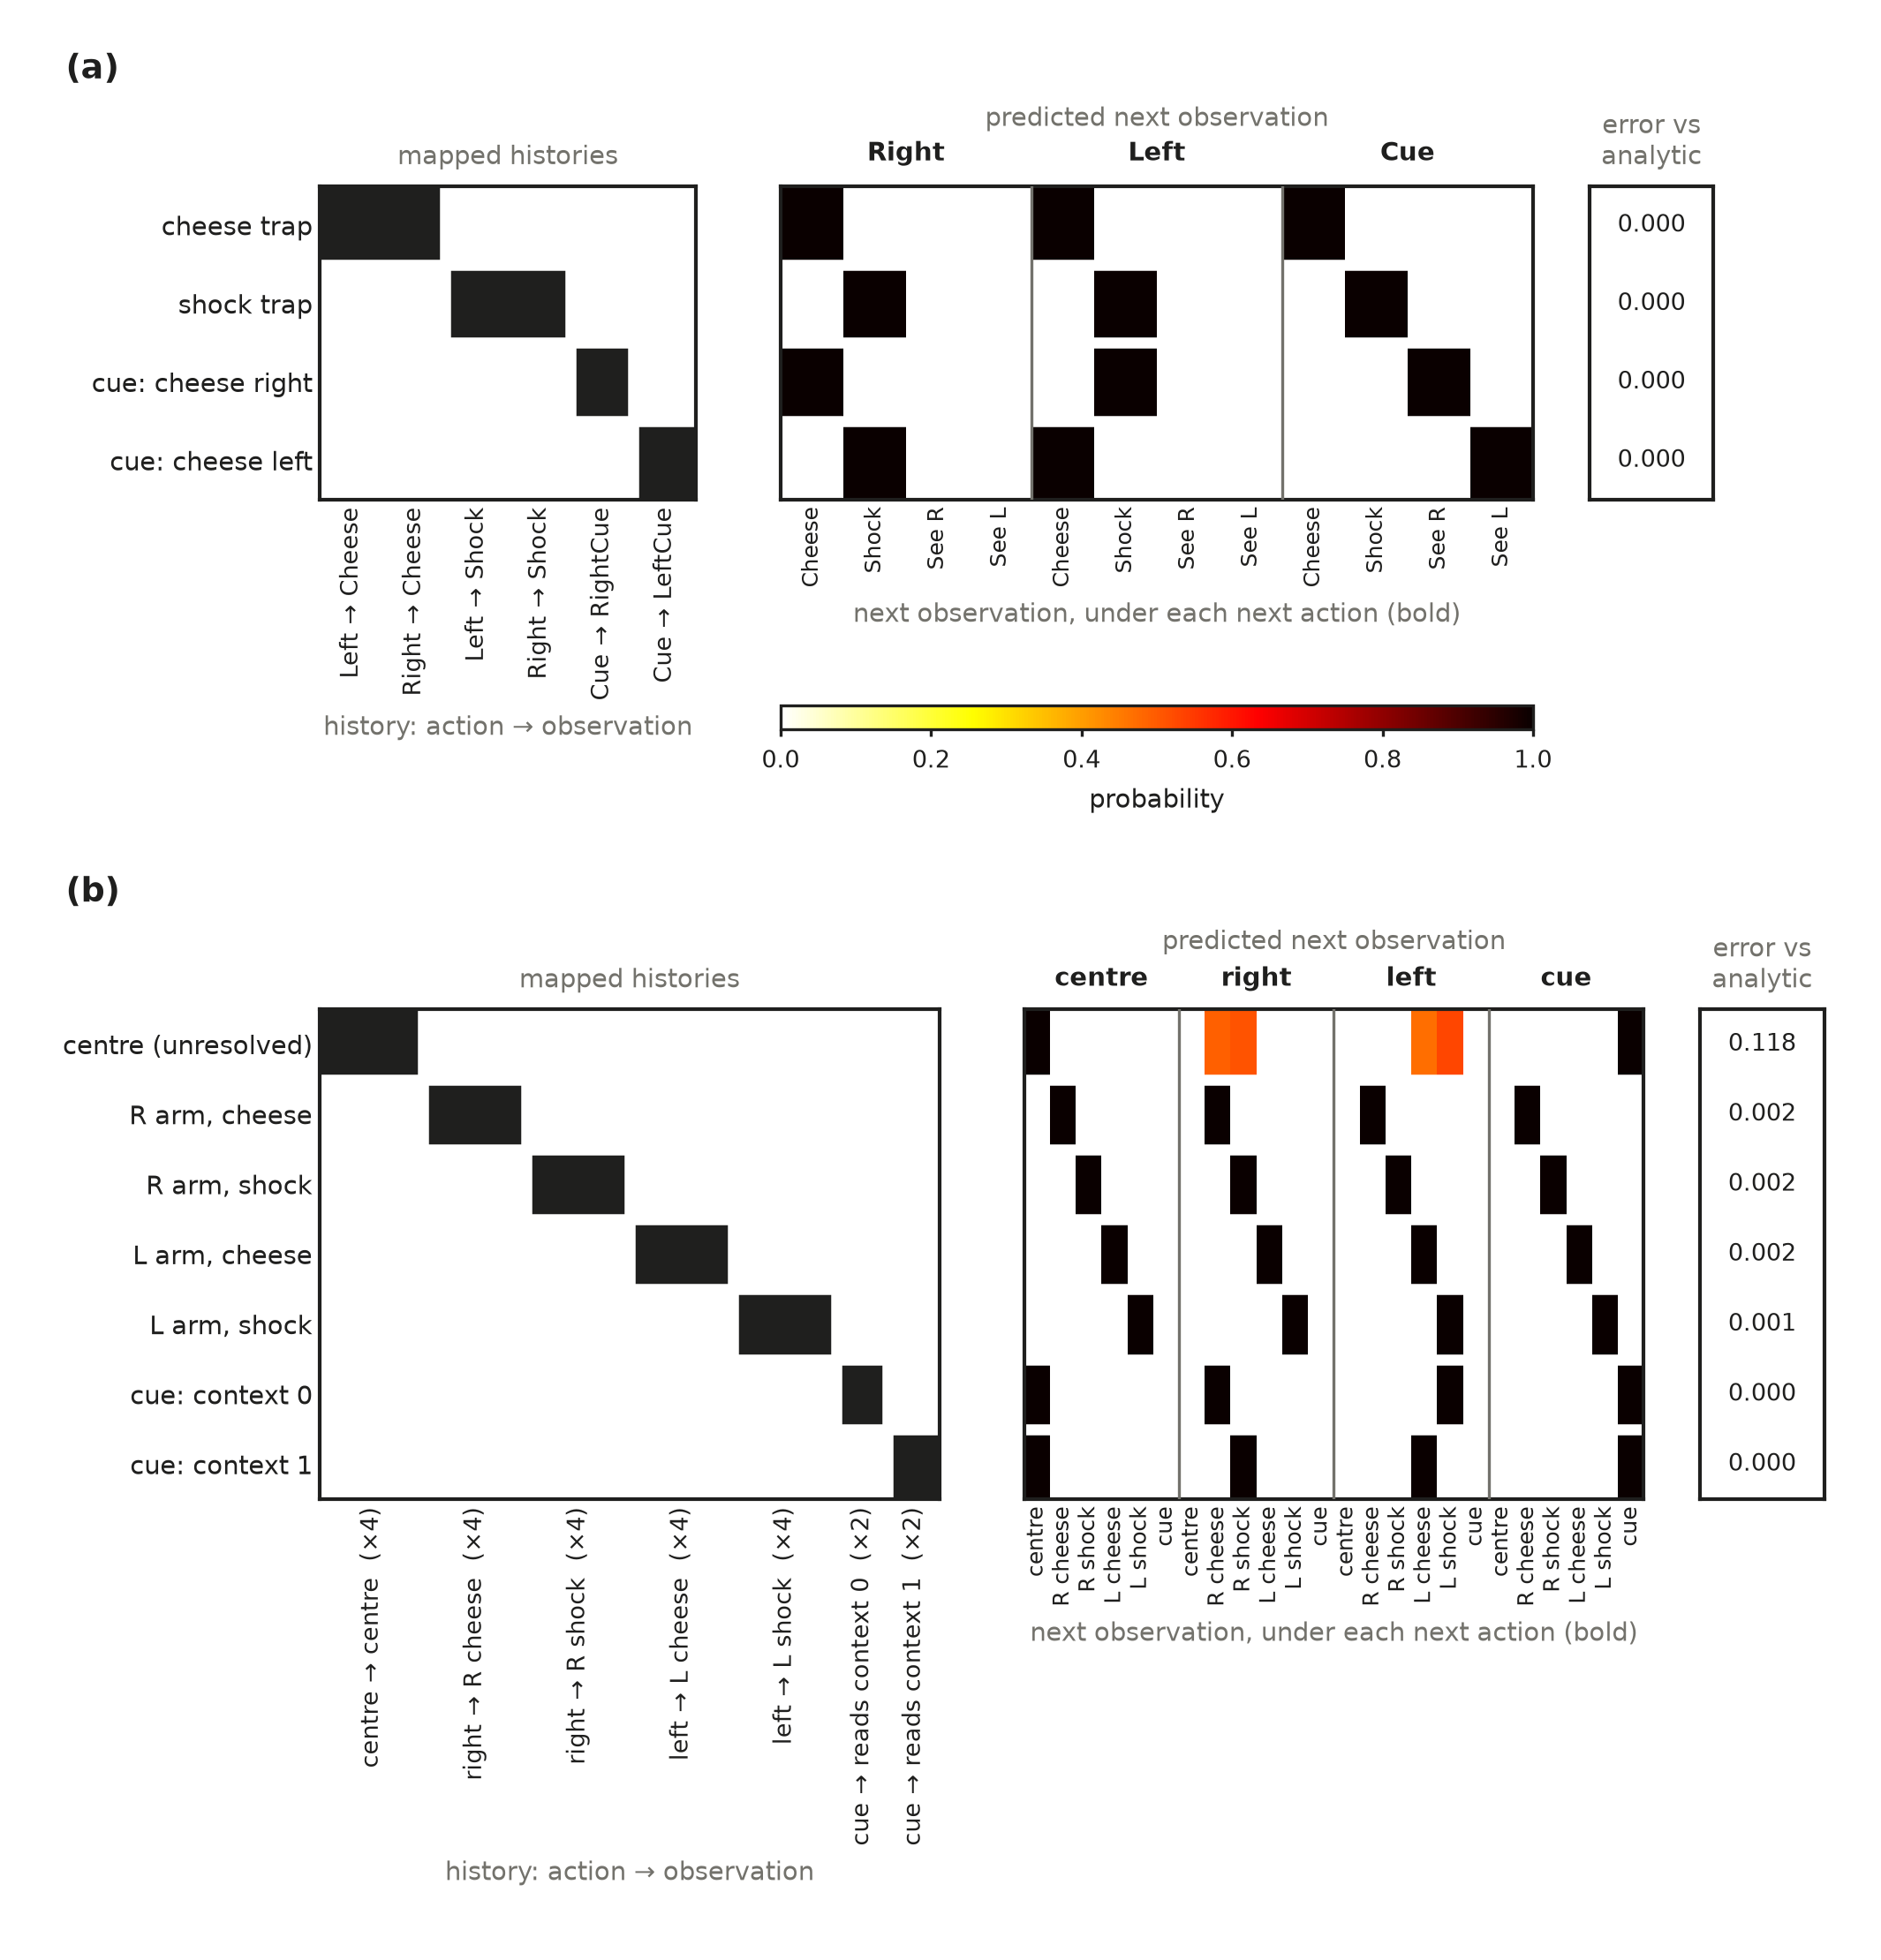
\includegraphics[width=0.92\textwidth]{Fig6.png}
\caption{The observation-to-hidden-state mapping that structure learning finds from behaviour alone (seed 0), which matches the four states we specified for the minimal maze. Each row is one hidden state selected by Bayesian model reduction on the learned tensor network. Left block: the mapping from histories (an action followed by the observation it produced) to states; a filled cell maps the history to the state. The mapping is certain: the Dirichlet evidence gives every history probability $p(\text{state} \mid \text{history}) > 1 - 10^{-22}$ for its own state in every seed. Structure learning reduces 6 histories to 4 states in the minimal maze and 24 to 7 in the pymdp T-maze. Middle block: what the state predicts, $p(o_{t+1} \mid \text{state}, a_{t+1})$, for each next action (bold), on the probability scale shown. Right column: the largest total-variation distance between a member history's learned prediction and the analytic one. (a) Minimal maze: the two arm-of-entry histories with the same outcome map to one trap state because position is unobservable, and the two cue readings map to one state each. (b) pymdp T-maze, over position and reward with the context modality marginalised. Every pymdp observation carries a context bit, which is random noise everywhere except at the cue. Each labelled history therefore occurs as several histories that differ only in these bits ($\times 4$, or $\times 2$ at the cue), and all of them map to the same state. At the cue the bit is the reading, and it separates the two cue states. Each trap predicts its own observation under every action, and each cue state predicts cheese in one arm and shock in the other. The unresolved centre predicts a fair outcome at either arm, and its error (0.118) is the sampling noise of its training counts, which the model reproduces.}
\label{fig:states}
\end{figure*}


\subsubsection{Implication for the main hypothesis} The learned models confirm the empowerment signature behind Proposition~\ref{prop:epistemic}. Its explanation as learning about the context, however, turns out to be a choice we made when specifying the state space by hand, and behaviour cannot certify it. The learned states are predictive states. They are the coarsest partition of histories that preserves every prediction, and in this two-step task they form the smallest state space at the bond that generates the data. The specified model of Section~\ref{sec:efe} distinguishes the choice point with the cheese on the left from the choice point with the cheese on the right. The learned model merges them, since no observation can tell them apart until the Cue is read. The same identifiability limit applies to information gain. The context model of Section~\ref{sec:efe} and a model in which an arm draws a fair outcome coin generate identical data, and they disagree on whether entering an arm is informative about the context. What the learned model does fix is that every action at the choice point resolves one bit about the next predictive state, either cheese-trap against shock-trap or one cue context against the other. It also fixes the net change in empowerment each action produces, $+0.58$ bits for the Cue and $-1$ bit for either arm, in every seed. The decomposition of Proposition~\ref{prop:epistemic} into an information term and an interface term depends on which latent variable is chosen, so it is a property of the specified model and not of behaviour; its sum is identifiable. For phenotyping, the signature of interface preservation can be read off a learned model: equal information gain with opposite changes in empowerment. Attributing that signature to learning about the context cannot be read off it.

The learned models phenotype control. They recover the channel and its latent structure. They do not recover the preferences or the causal chain from beliefs to action that the criteria of Section~\ref{sec:definition} require, so the learned-model results are control phenotyping. Agency phenotyping proper needs inverse inference of preferences, which is future work. The pipeline also identifies the interventional channel $p(o_{t+1} \mid \mathrm{do}(a_t))$ from observational data only under a stated condition, that the rollouts give every action full support at every reachable state, chosen independently of the system's own policy. Our rollouts are sampled under a uniform-action policy, so the condition holds. For data generated by a competent policy it fails, since such a policy never takes the uninformative actions whose consequences the channel needs; the companion repository includes a check, computed from the data alone, of whether the condition holds.

\begin{table*}[t]
\centering
{\small
\begin{tabular}{lcccc}
\hline
 & \multicolumn{2}{c}{\textbf{Minimal maze}} & \multicolumn{2}{c}{\textbf{pymdp T-maze, reward}} \\
\textbf{Condition} & analytic & learned & analytic & learned \\
\hline
Start ($t_1$) & 1.000 & 1.002 $\pm$ 0.002 & 1.000 & 1.000 $\pm$ 0.001 \\
Trapped & 0 & 0.000 $\pm$ 0.000 & 0 & 0.000 $\pm$ 0.000 \\
Post-cue & 1.585 & 1.585 $\pm$ 0.000 & 1.585 & 1.583 $\pm$ 0.002 \\
\hline
$L_1$ to analytic & & 0.218 $\pm$ 0.025 & & 0.193 $\pm$ 0.011 \\
$L_1$ floor (held-out) & & 0.240 $\pm$ 0.035 & & 0.396 $\pm$ 0.016 \\
Held-out NLL (model / true) & & 2.909 / 2.890 & & 5.274 / 5.242 \\
States, BMR (minimal model) & & 4.0 $\pm$ 0.0 (4) & & 7.0 $\pm$ 0.0 (7) \\
States, plain fidelity & & 4.4 $\pm$ 0.5 & & 11.3 $\pm$ 1.5 \\
\hline
\end{tabular}
}
\caption{Empowerment (bits) and fit of tensor networks trained on sampled rollouts, mean $\pm$ SD over 5 seeds (minimal maze) and 3 seeds (pymdp T-maze, reward modality; the full observation space gives 2.000 / 0 / 2.000 analytically and 2.000 / 0.007 / 1.998 learned). Trapped and post-cue values are averaged over contexts. The $L_1$ floor is the distance between the analytic joint and the held-out empirical joint of the same seed. NLL is the held-out negative log-likelihood per trajectory in nats, against the entropy of the true process. States are predictive states selected by Bayesian model reduction at $\alpha = 0.1$ (pymdp T-maze: over position and reward), unchanged for $10^{-3} \le \alpha \le 0.5$; in parentheses, the size of the smallest model that generates the data. Plain fidelity is computed over all supported histories.}
\label{tab:learned}
\end{table*}

\section{Discussion and Conclusions}\label{sec:discussion}

Notions of agency matter for how we explain others' actions, ascribe responsibility, and determine which actions should be permitted. As AI systems operate with increasing independence, policymakers must wrestle with how to govern systems that set their own priorities and decide without direct human control, what we call the \emph{agency problem of AI governance}.

\subsection{Governance: From Conclusions to a Research Agenda.}

Governance of autonomous agents is an established research programme in multi-agent systems, and our hypotheses should be read against it. \citet{pittAxiomatizationSocioEconomic2012} axiomatise Ostrom's principles for self-governing institutions in the Event Calculus and study when self-organised resource allocation among autonomous agents is sustainable; \citet{pittComputationalJustice2015} and \citet{pittOpenAgentSociety2015} extend this to computational justice in open systems, and \citet{pittSelfOrganisingMAS2021} collects the programme; \citet{singhNormsGoverning2013} grounds governance in computational norms among agents whose internals are opaque to one another. These programmes take the agents' control over the shared resource as a design given and ask what conventional rules make collective self-governance work. Our proposal is complementary and narrower. It supplies a measured variable, the agent's controllability over its own interface, and predicts which class of governance handle (structural constraint, external contingency, or modulation of internal preferences) remains effective as that variable grows. H1--H3 state that prediction.

The worked example suggests, but does not establish, a mapping from control regimes to governance handles: external structural controls in the zero-control regime, preference shaping in the intermediate regime, and intervention on the agent's internal preferences and model in the maximal regime. We offer this as a research agenda of falsifiable hypotheses, testable in larger environments and, via Section~\ref{sec:learned}, on learned models of non-active-inference systems:
\begin{itemize}
    \item \textbf{H1 (Measurement validity).} An empowerment estimate read off a learned model is valid if it predicts the effects of interventions. Where the estimate is zero, changing the agent's preferences or beliefs should leave outcomes unchanged; elsewhere the effect of such a change, measured as the total-variation distance between the outcome distributions under the two profiles, should grow with the estimate. \emph{Falsified if} interventions produce effects at estimated-zero states, which would show that the estimator uses the wrong modalities, horizon or model.
    \item \textbf{H2 (Crossover).} As empowerment increases, external-constraint interventions lose effect size relative to preference-modulating ones, with effect size measured as in H1 and the ordering tested across states ranked by empowerment. \emph{Falsified if} external constraints stay uniformly dominant, or no ordering by empowerment exists.
    \item \textbf{H3 (Epistemic escalation).} Agents that minimise expected free energy tend to select interface-preserving epistemic actions (Proposition~\ref{prop:epistemic}) and so move toward higher-empowerment states, and static controllability assessments then underestimate future controllability. The T-maze isolates two routes with separate conditions. The epistemic route operates when the epistemic action is the more reliable source of the same information (Section~\ref{sec:noisyarm}), the preference route when the alternatives are aversive or the resolved belief has decision value within the planning horizon (Sections~\ref{sec:efe} and~\ref{sec:twostep}). \emph{Testable} by manipulating source reliabilities and preference profiles independently in EFE-minimising agents and reward-only baselines. \emph{Falsified if} empowerment does not rise under the epistemic route with preferences flat.
\end{itemize}

\subsection{Limitations}
Empowerment measures controllability. Reading it as an agency regime requires independent access to the agent's beliefs and desires (Section~\ref{sec:notagency}), and our ``subjective potential empowerment'' departs from true, objective, or actual empowerment. Rationality is relative to the generative model, so the criterion is informative only alongside an independent assessment of whether the model fits the environment. Treating autonomy as intentional independence and adaptivity as rationality's signature is a choice of terms made for brevity (Section~\ref{sec:definition}) and does not claim that the concepts are identical. Finally, all results come from a two-step discrete POMDP. Scaling up requires variational empowerment estimators~\citep{mohamedVariationalInformationMaximisation2015}, the model-learning step of Section~\ref{sec:learned}, and the same observation modalities across comparisons, since empowerment depends on how observations are represented. Suitable estimators include those that are stable in continuous control~\citep{zhaoEfficientEmpowerment2021} and representation-learning formulations~\citep{choiVariationalEmpowerment2021}. Deep active inference agents~\citep{fountasDeepActiveInference2020} are the natural first systems to phenotype, since both the probe and the criteria apply to them directly. The paper defines the measurements a demonstration at scale would need and does not provide one.

\subsection{Conclusion}

The contribution of this paper is mainly conceptual. It gives a three-criterion definition of agency (intentionality, rationality, explainability) that is grounded in philosophy and can be operationalised. It argues that active inference realises all three criteria together under a single normative objective, in a way that can be compared across architectures (Table~\ref{tab:frameworks}). It also gives a controlled illustration in a minimal POMDP. There, empowerment, used strictly as a probe of controllability, tracks structural changes to the agentic action chain. Epistemic actions that keep the interface intact increase empowerment, and expected free energy minimisation selects such actions without empowerment being an explicit objective. It does so through preferences in the deterministic maze, and through the epistemic term as soon as the epistemic action is the more reliable source of the context. Tensor networks trained on behaviour alone, using an observable fidelity and Bayesian model reduction, recover the hidden states we specified for the minimal maze and discover those of the pymdp T-maze, the smallest state spaces that generate the data. They also show that the context variable of our information-gain analysis is not one that behaviour supports. They confirm the signature of interface preservation: equal information gain about the next state with opposite changes in empowerment. They also show that attributing this signature to learning about the context is a property of the specified state space, and behaviour cannot certify it. Whether this becomes phenotyping in the full sense depends on the programme of Section~\ref{sec:learned}, which fits generative models to the behaviour of real AI systems and checks the inferred agency profiles against the interventions of H1--H3.

% \section*{Reproducibility}
% Code for the active inference T-maze experiments, the agency metrics, and the tensor-network pipeline of Section~\ref{sec:learned} is provided as supplementary material and will be released in public repositories upon publication. (Links withheld for anonymous review.)
\bibliography{references}

\begin{appendices}

\section{Proofs}\label{app:proofs}

\paragraph{Setting.}
At a decision point the agent has a finite action set $\cA$ and observation set $\cO$. The hidden state $s \in \cS$ is unknown; the agent holds a belief $q \in \Delta(\cS)$. For each $s$ the one-step consequence of acting is a row-stochastic matrix $W_s \in \cW \subset \R^{|\cA| \times |\cO|}$, $W_s(o \mid a) = p(o_{t+1} = o \mid a_t = a, s)$. We call the triple $(\cA, \cO, \{W_s\}_{s \in \cS})$ the agent's \emph{interface}. The \emph{belief-averaged channel} is
\begin{equation}
  \bar W_q \;=\; \sum_{s \in \cS} q(s)\, W_s ,
  \label{eq:mixed}
\end{equation}
which is the conditional $p(o_{t+1} \mid a_t)$ that an agent with belief $q$ actually predicts. For a channel $W$ write $I(p; W)$ for the mutual information between an input distributed as $p \in \Delta(\cA)$ and the output, and $\Capa(W) = \max_{p} I(p; W)$ for its capacity. The subjective potential empowerment of Section~\ref{sec:metric} under belief $q$ is
\begin{equation}
  \Emp(q) \;=\; \Capa(\bar W_q).
  \label{eq:emp}
\end{equation}

\begin{lemma}[Capacity is convex in the channel]
\label{lem:convex}
$\Capa : \cW \to \R$ is convex.
\end{lemma}
\begin{proof}
For fixed input distribution $p$, $I(p; W)$ is a convex function of the channel $W$~\citep[Theorem~2.7.4]{coverElementsInformationTheory2006}. A pointwise maximum of convex functions is convex, and $\Capa(W) = \max_p I(p; W)$.
\end{proof}

\begin{lemma}[Updating at a fixed interface never lowers expected empowerment]
\label{lem:update}
Let the agent perform any experiment before acting, receiving an observation $y \in \mathcal{Y}$ drawn from $p(y \mid s)$, with posterior $q_y(s) \propto q(s)\, p(y \mid s)$ and marginal $p(y) = \sum_s q(s)\, p(y \mid s)$. If the interface is unchanged by the experiment, then
\begin{equation}
  \E_{y \sim p(y)}\big[\Emp(q_y)\big] \;\ge\; \Emp(q).
  \label{eq:update}
\end{equation}
\end{lemma}
\begin{proof}
By the law of total probability, $\sum_y p(y)\, \bar W_{q_y} = \sum_y p(y) \sum_s q_y(s) W_s = \sum_s \big(\sum_y p(y) q_y(s)\big) W_s = \sum_s q(s) W_s = \bar W_q$. Apply Jensen's inequality to the convex function $\Capa$ of Lemma~\ref{lem:convex}: $\Capa(\bar W_q) = \Capa\big(\sum_y p(y) \bar W_{q_y}\big) \le \sum_y p(y)\, \Capa(\bar W_{q_y})$.
\end{proof}

\begin{corollary}[Full resolution]
\label{cor:resolve}
If the experiment reveals $s$ exactly, then $\E_{s \sim q}\big[\Capa(W_s)\big] \ge \Capa(\bar W_q)$. The empowerment an agent computes under a mixed belief is a lower bound on the empowerment it expects to have once the hidden state is known, at the same interface.
\end{corollary}

\paragraph{The T-maze instance.}
Let $\cS = \{L, R\}$ be the cheese location, $q = (\tfrac12, \tfrac12)$, $\cA = \{\text{Left}, \text{Right}, \text{Cue}\}$ and $\cO = \{\text{Cheese}, \text{Shock}, \text{SeeLeft}, \text{SeeRight}\}$. Under context $L$ the three rows of $W_L$ are the point masses on Cheese, Shock, SeeLeft; under $R$ they are Shock, Cheese, SeeRight. Each $W_s$ has three distinct deterministic rows, so $\Capa(W_s) = \log_2 3$. The mixed channel $\bar W_q$ has rows $(\tfrac12, \tfrac12, 0, 0)$, $(\tfrac12, \tfrac12, 0, 0)$ and $(0, 0, \tfrac12, \tfrac12)$. Left and Right are indistinguishable and $\Capa(\bar W_q) = 1$ bit. Corollary~\ref{cor:resolve} reads $\log_2 3 \approx 1.585 \ge 1$, with strict inequality. These are the baseline and post-Cue values of the main text.

\begin{proof}[Proof of Proposition~\ref{prop:epistemic}]
An action $a$ does two things at once. It yields an observation, which updates the belief from $q$ to $q_y$, and it moves the agent to a possibly different interface with channel family $\{W'_s\}$ and empowerment functional $\Emp'$. The expected change in empowerment decomposes as
\begin{equation}
  \E_y\big[\Emp'(q_y)\big] - \Emp(q)
  \;=\;
  \underbrace{\E_y\big[\Emp(q_y)\big] - \Emp(q)}_{\text{information term}}
  \;+\;
  \underbrace{\E_y\big[\Emp'(q_y) - \Emp(q_y)\big]}_{\text{interface term}} .
  \label{eq:decomp}
\end{equation}
The information term is non-negative by Lemma~\ref{lem:update}. The interface term has no sign in general. If the interface is intact ($W'_s = W_s$ for all $s$, up to relabelling of actions and observations), the interface term is zero and the gain equals the information term, which is strictly positive whenever the resolved channels have larger capacity than the mixed one, as they do in the T-maze. Separating a merged pair of rows is not by itself enough. In the T-maze the Cue resolves the context and returns the agent to the same three-way choice, so its interface term is zero and its information term is $\log_2 3 - 1$ bits. Either arm resolves the context equally well (its information term is the same $\log_2 3 - 1$ bits) but enters an absorbing state whose channel has identical rows, so its interface term is $0 - \log_2 3$ and the net change is $-1$ bit. A construction in which an action reveals the hidden state and disables the interface has the same structure, a zero information term because the actions were already distinguishable and a negative interface term.
\end{proof}

\begin{definition}[$n$-step empowerment]
For a horizon $n \ge 1$, an interface and belief $q$,
\begin{equation}
  \Emp_n(q) \;=\; \max_{p(a_{1:n})}\; I\big(A_{1:n};\, O_{2:n+1}\big),
\end{equation}
the capacity from open-loop action sequences of length $n$ to the resulting observation sequences, with $o_{t+1}$ the observation that follows $a_t$, under the agent's predictive model. $\Emp_1 = \Emp$ of~\eqref{eq:emp}. By the chain rule $\Emp_n \ge \max_p I(A_{1:n}; O_{n+1})$, the endpoint form of~\citet{Klyubin2005empowerment}.
\end{definition}

\begin{proof}[Proof of Proposition~\ref{prop:zero}]
Capacity zero at horizon $n$ means $I(A_{1:n}; O_{2:n+1}) = 0$ for every input distribution, in particular for one with full support, so $p(o_{2:n+1} \mid a_{1:n})$ does not depend on $a_{1:n}$. Zero capacity at the horizon $T$ alone already gives the shorter cases by marginalisation. A closed-loop policy selects $a_k$ as a function of $o_{2:k}$. By induction on $k$ the distribution of $o_{2:k+1}$ is the same under every such policy, because $p(o_{k+1} \mid o_{2:k}, a_{1:k})$ is action-independent by the $n = k$ case and $o_{2:k}$ does not depend on $a_k$. For the last claim take two actions $a_0$ and $a_1$ that both yield $o_1 = c$ but lead to $s_0$ and $s_1$, which $o_2$ distinguishes: $\Emp_1 = 0$ while $\Emp_2 \ge I(A_1; O_2) = 1$ bit.
\end{proof}

\paragraph{Actual empowerment under a stochastic policy.}
Actual empowerment is the mutual information $I(p; \bar W_q)$ evaluated at the agent's own action distribution $p$ instead of maximised over $p$. It is identically zero for a deterministic policy, but an active inference agent's policy is not deterministic. Action selection is a softmax over negative expected free energy with precision $\gamma$, $p_\gamma(a) \propto \exp\{-\gamma\, G(a)\}$, so actual empowerment
\begin{equation}
  \Emp^{\mathrm{act}}_\gamma(q) \;=\; I\big(p_\gamma;\, \bar W_q\big)
\end{equation}
is a continuous function of $\gamma$ with $\Emp^{\mathrm{act}}_\gamma \to 0$ as $\gamma \to \infty$ when the minimiser of $G$ is unique, and $\Emp^{\mathrm{act}}_\gamma \to I(\text{uniform}; \bar W_q) \le \Emp(q)$ as $\gamma \to 0$. It is degenerate only in the infinite-precision limit. In the T-maze at the choice point with $C = (2, -4, 0, 0)$ and $\gamma = 16$, the policy posterior is effectively the point mass on Cue and actual empowerment is $0.000$ bits against a potential of $1$ bit; with flat preferences it is $0.918$ bits.

\end{appendices}

\end{document}
